\documentclass[12pt]{article}
\usepackage[spanish]{babel}
\usepackage{geometry}
\geometry{a4paper, margin=1in}
\usepackage{graphicx}
\usepackage{xcolor}
\usepackage{titlesec}
\usepackage{parskip}
\usepackage{multicol}
\usepackage{cite}
\usepackage{float}
\usepackage{amsmath}

\definecolor{highlight}{RGB}{255, 255, 0}

\titleformat{\section}{\normalfont\Large\bfseries}{\thesection}{1em}{}
\titleformat{\subsection}{\normalfont\large\bfseries}{\thesubsection}{1em}{}

\begin{document}

% Logos
\begin{minipage}{0.45\textwidth}
    
\includegraphics[width=0.4\textwidth]{inFiles/Figures/epnLogo.jpg}
\end{minipage}
\hfill
\begin{minipage}{0.45\textwidth}
    \raggedleft
    
\includegraphics[width=0.4\textwidth]{inFiles/Figures/FIS_logo.jpg}
\end{minipage}

\vspace{0.5cm}

% Títulos principales
\begin{center}
    \textbf{ESCUELA POLITÉCNICA NACIONAL}\\[0.2cm]
    \textbf{FACULTAD DE INGENIERÍA DE SISTEMAS}\\[0.2cm]
    \textbf{INGENIERÍA {\textbf{EN COMPUTACIÓN}}}
\end{center}

\vspace{0.5cm}
\hrule
\vspace{0.5cm}

% Datos principales
\noindent\textbf{PERÍODO ACADÉMICO:} 2025-A\\[0.2cm]
\noindent\textbf{ASIGNATURA:} ICCD412 Métodos Numéricos \hfill \textbf{GRUPO:} GR2\\[0.2cm]
\noindent\textbf{TIPO DE INSTRUMENTO:} Repaso 3\\[0.2cm]
\noindent\textbf{FECHA DE ENTREGA LÍMITE:} 8/07/2025\\[0.2cm]
\noindent\textbf{ALUMNO:} Murillo Tobar Juan

\vspace{0.5cm}
\hrule
\vspace{1cm}


% Secciones
\section*{TEMA}
Repaso

\vspace{0.5cm}

\section*{OBJETIVOS}
\begin{itemize}
    \item Utilizar el método de Gauss para la  resolución de sistemas de ecuaciones lineales.
    \item Utilizar el método de Gauss Jordan para la resolución de sistemas de ecuaciones lineales.
    \item Utilizar factorización de matrices para la resolución de sistemas de ecuaciones lineales. 
\end{itemize}

\vspace{0.5cm}


\section*{DESARROLLO}

\begin{figure}[H]
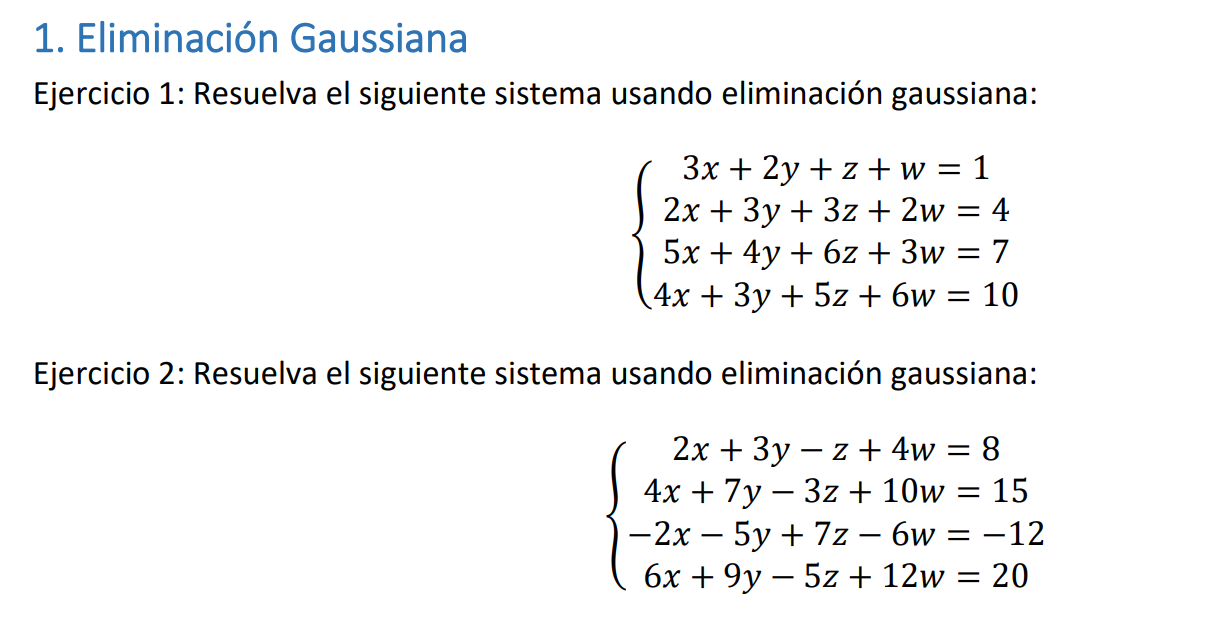
\includegraphics[width=1\textwidth]{./inFiles/Figures/Ej1.png}
\end{figure}

\textbf{a)}
\[
\begin{bmatrix}
3 & 2 & 1 & 1 & 1\\
2 & 3 & 3 & 2 & 4 \\
5 & 4 & 6 & 3 & 7 \\
4 & 3 & 5 & 6 & 10
\end{bmatrix}
\]
-2*F1+3*F2 $\longrightarrow $ F2

-5*F1+3*F3 $\longrightarrow $ F3

-4*F1+3*F4 $\longrightarrow $ F4

\[
\begin{bmatrix}
3 & 2 & 1 & 1 & 1\\
0 & 5 & 7 & 4 & 10 \\
0 & 2 & 13 & 4 & 16 \\
0 & 1 & 11 & 14 & 26
\end{bmatrix}
\]

Cambio de filas F4 con F2

\[
\begin{bmatrix}
3 & 2 & 1 & 1 & 1\\
0 & 1 & 11 & 14 & 26\\
0 & 2 & 13 & 4 & 16 \\
0 & 5 & 7 & 4 & 10 \\
\end{bmatrix}
\]

-2*F2+F3 $\longrightarrow $ F3

-5*F2+F4 $\longrightarrow $ F4

\[
\begin{bmatrix}
3 & 2 & 1 & 1 & 1\\
0 & 1 & 11 & 14 & 26\\
0 & 0 & -9 & -24 & -36 \\
0 & 0 & -48 & -66 & -120 \\
\end{bmatrix}
\]

-16/3*F3+F4 $\longrightarrow $ F4

\[
\begin{bmatrix}
3 & 2 & 1 & 1 & 1\\
0 & 1 & 11 & 14 & 26\\
0 & 0 & -9 & -24 & -36 \\
0 & 0 & 0 & 62 & 72 \\
\end{bmatrix}
\]

Haciendo la substitución para atrás Y redondeando obtenemos
$X4 = 36/31$ $X3 = 28/31$    $X2 = -6/31$  $X1 = -7/31$ 




\textbf{b)}
\[
\begin{bmatrix}
2 & 3 & -1 & 4 & 8\\
4 & 7 & -3 & 10 & 15 \\
-2 & -5 & 7 & -6 & -12 \\
6 & 9 & -5 & 12 & 20
\end{bmatrix}
\]
-2*F1+F2 $\longrightarrow $ F2

F1+F3 $\longrightarrow $ F3

-3*F1+F4 $\longrightarrow $ F4

\[
\begin{bmatrix}
2 & 3 & -1 & 4 & 8\\
0 & 1 & -1 & 2 & -1 \\
0 & -2 & 6 & -2 & -4 \\
0 & 0 & -2 & 0 & -4
\end{bmatrix}
\]

Cambio de filas F4 con F3

\[
\begin{bmatrix}
2 & 3 & -1 & 4 & 8\\
0 & 1 & -1 & 2 & -1 \\
0 & 0 & -2 & 0 & -4
0 & -2 & 6 & -2 & -4 \\

\end{bmatrix}
\]

2*F2+F4 $\longrightarrow $ F4


\[
\begin{bmatrix}
2 & 3 & -1 & 4 & 8\\
0 & 1 & -1 & 2 & -1 \\
0 & 0 & -2 & 0 & -4
0 & 0 & 4 & 2 & -6 \\

\end{bmatrix}
\]

2F3+F4 $\longrightarrow $ F4

\[
\begin{bmatrix}
2 & 3 & -1 & 4 & 8\\
0 & 1 & -1 & 2 & -1 \\
0 & 0 & -2 & 0 & -4
0 & 0 & 0 & 2 & -14 \\

\end{bmatrix}
\]

Haciendo la substitución para atrás Y redondeando obtenemos
$X4 = -7$ $X3 = 2$    $X2 = 15$  $X1 = -7/2$ 


\begin{figure}[H]
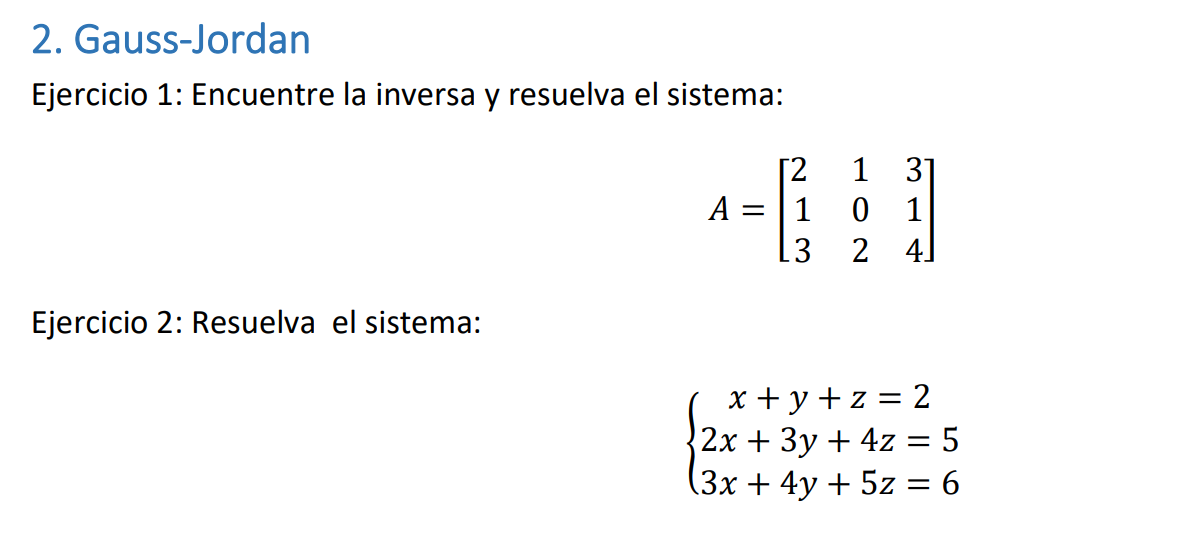
\includegraphics[width=1\textwidth]{./inFiles/Figures/Ej2.png}
\end{figure}

\textbf{a)}
\[
\begin{bmatrix}
2 & 1 & 3 & 1& 0& 0\\
1 & 0 & 1 & 0& 1& 0\\
3 & 2 & 4 & 0& 0& 1\\
\end{bmatrix}
\]

Cambio de fila F1 con F2

\[
\begin{bmatrix}
1 & 0 & 1 & 0& 1& 0\\
2 & 1 & 3 & 1& 0& 0\\
3 & 2 & 4 & 0& 0& 1\\
\end{bmatrix}
\]


-2*F1+F2 $\longrightarrow $ F2

-3*F1+F3 $\longrightarrow $ F3

\[
\begin{bmatrix}
1 & 0 & 1 & 0& 1& 0\\
0 & 1 & 1 & 1& -2& 0\\
0 & 2 & 1 & 0& -3& 1\\
\end{bmatrix}
\]

-2*F2+F3 $\longrightarrow $ F3

\[
\begin{bmatrix}
1 & 0 & 1 & 0& 1& 0\\
0 & 1 & 1 & 1& -2& 0\\
0 & 0 & -1 & -2& 1& 1\\
\end{bmatrix}
\]

F3+F1 $\longrightarrow $ F1

F2+F3 $\longrightarrow $ F2

-F3 $\longrightarrow $ F3

\[
\begin{bmatrix}
1 & 0 & 0& -2& 2& 1\\
0 & 1 &  0& -1& -1& 1\\
0 & 0 & 1 & 2& -1& -1\\
\end{bmatrix}
\]


\textbf{b)}

\[
\begin{bmatrix}
1 & 1 & 1& 2\\
2 & 3 & 4& 5\\
3 & 4 & 5& 6\\
\end{bmatrix}
\]

-2F1 +F2 $\longrightarrow $ F2

-3F1+F3 $\longrightarrow $ F3

\[
\begin{bmatrix}
1 & 1 & 1& 2\\
0 & 1 & 2& 1\\
0 & 1 & 2& 0\\
\end{bmatrix}
\]

-F2+F3 $\longrightarrow $ F3

\[
\begin{bmatrix}
1 & 1 & 1& 2\\
0 & 1 & 2& 1\\
0 & 0 & 0& -1\\
\end{bmatrix}
\]

No hay solución

\begin{figure}[H]
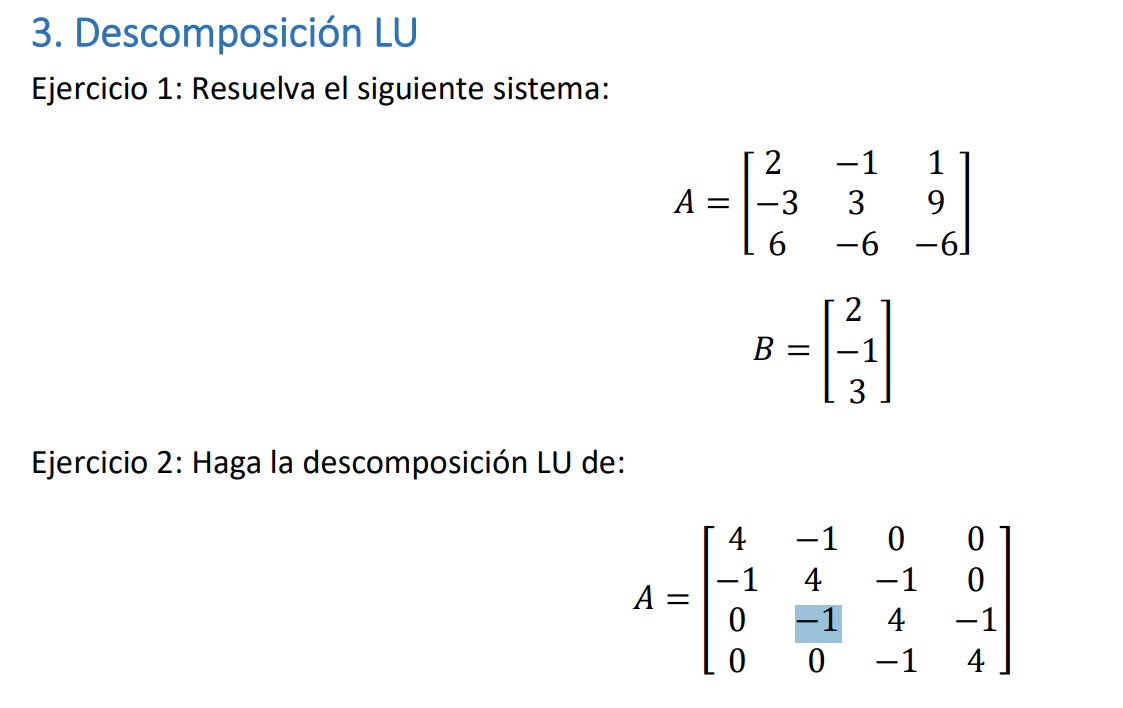
\includegraphics[width=1\textwidth]{./inFiles/Figures/Ej3.png}
\end{figure}


\textbf{a)}

Usando las formulas obtenemos

u11 = 2

u12 = -1

u13 = 1

u22 = 3/2

u23 = 21/2

u33  = 9

l21 = -3/2

l31 = 3

l32 = -2


\[
\begin{bmatrix}
1 & 0 & 0\\
-3/2 &  1& 0\\
3 & -2 & 1\\
\end{bmatrix}
*
\begin{bmatrix}
2 & -1 & 1\\
0 & 3/2 & 21/2\\
0 & 0 & 12\\
\end{bmatrix}
\]

Ahora calculamos y con Ly=b

\[
\begin{bmatrix}
1 & 0 & 0& 2\\
-3/2 &  1& 0& -1\\
3 & -2 & 1& 3\\
\end{bmatrix}
\]


Haciendo la substitución para adelante Y redondeando obtenemos
$y1 = 2$    $y2 =2$  $y3 =1$ 

Ahora x con Ux = y
\[
\begin{bmatrix}
2 & -1 & 1& 2\\
0 & 3/2 & 21/2& 2\\
0 & 0 & 12& 1\\
\end{bmatrix}
\]

Haciendo la substitución para atrás obtenemos
$x1 = 4/3$    $x2 = 3/4$  $x3 =1/12$ 



\textbf{b)}

En este caso pondré todas las formulas y luego los resultados, usaremos Doolittle

u11 = A11; u12 = A12;  u13 = A13; u14 = A14

l21 = A21/u11; l31 = A31/u11; l31 = A41/u11

u22 = A22 - l21*u12

u23 = A23 - l21*u13

u24 = A24 - l21*u14

l32 = (A32 - l31*u12)/u22

l42 = (A42 - l41*u12)/u22

u33 = A33-l31*u13-l32*u23

u34 = A34 - l31*u14 -l32*u24

l44 = (A43 - l41*u12-l42*u23)/u33

u44 = A44 - l41*u14 -l42*u24 -l43*u34

\[
\begin{bmatrix}
1 & 0 & 0& 0\\
-1/4 & 1 & 0& 0\\
0 & -4/15 & 1& 0\\
0 & 0 & -15/56& 1\\
\end{bmatrix}
*
\begin{bmatrix}
4 & -1 & 0& 0\\
0 & 15/4 & -1& 0\\
0 & 0 & 56/15& -1\\
0 & 0 & 0& 209/56\\
\end{bmatrix}
\]





\begin{figure}[H]
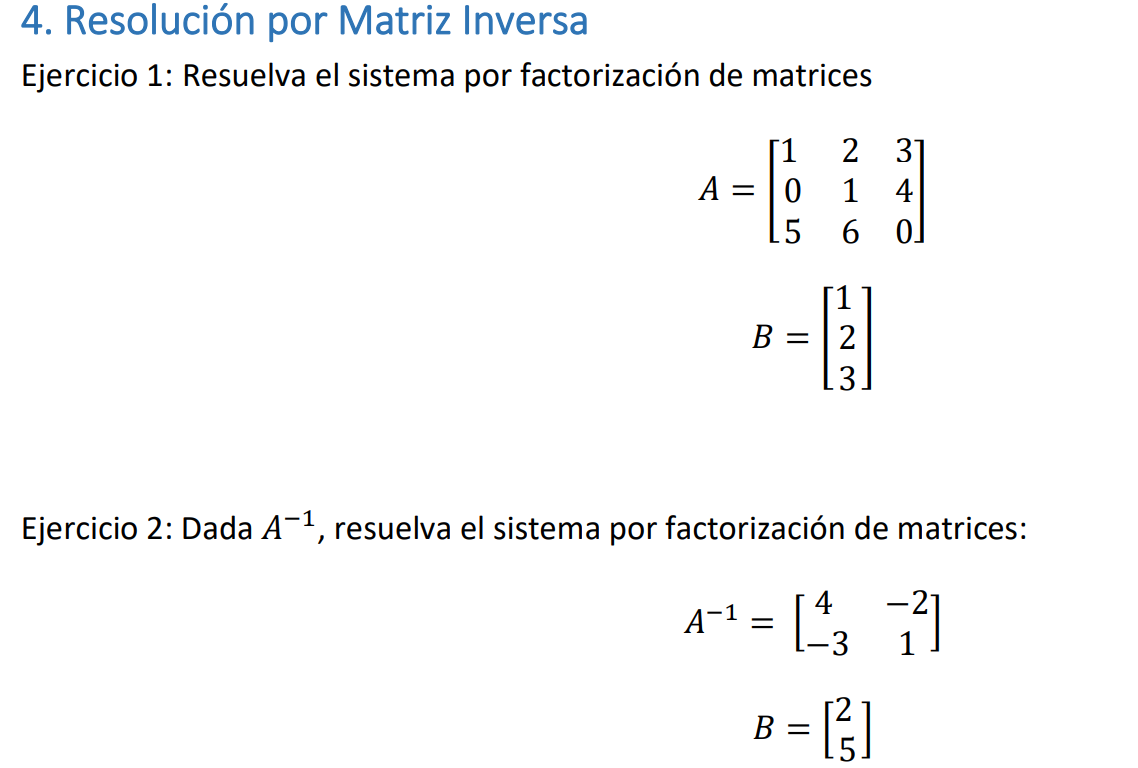
\includegraphics[width=1\textwidth]{./inFiles/Figures/Ej4.png}
\end{figure}


\textbf{a)}
Hallamos la matriz inversa de A

\[
\begin{bmatrix}
1 & 2 & 3 & 1& 0& 0\\
0 & 1 & 4 & 0& 1& 0\\
5 & 6 & 0 & 0& 0& 1\\
\end{bmatrix}
\]

-5*F1+F3 $\longrightarrow $ F3

\[
\begin{bmatrix}
1 & 2 & 3 & 1& 0& 0\\
0 & 1 & 4 & 0& 1& 0\\
0 & -4 & -15 & -5& 0& 1\\
\end{bmatrix}
\]

4*F2+F3 $\longrightarrow $ F3

\[
\begin{bmatrix}
1 & 2 & 3 & 1& 0& 0\\
0 & 1 & 4 & 0& 1& 0\\
0 & 0& 1 & -5& 4& 1\\
\end{bmatrix}
\]

-4*F3+F2 $\longrightarrow $ F2

-3*F3+F1 $\longrightarrow $ F1


\[
\begin{bmatrix}
1 & 2 & 0 & 16& -12& -3\\
0 & 1 & 0 & 20& -15& -4\\
0 & 0& 1 & -5& 4& 1\\
\end{bmatrix}
\]

-2*F2+F1 $\longrightarrow $ F1

\[
\begin{bmatrix}
1 & 0 & 0 & -24& 18& 5\\
0 & 1 & 0 & 20& -15& -4\\
0 & 0& 1 & -5& 4& 1\\
\end{bmatrix}
\]

Multiplico por b
\[
\begin{bmatrix}
-24& 18& 5\\
20& -15& -4\\
-5& 4& 1\\
\end{bmatrix}
*
\begin{bmatrix}
1\\
2\\
3\\
\end{bmatrix}
=
\begin{bmatrix}
27\\
-22\\
6\\
\end{bmatrix}
\]

\textbf{b)}

Multiplico por b
\[
\begin{bmatrix}
4& -2\\
-3& 1\\
\end{bmatrix}
*
\begin{bmatrix}
2\\
5\\
\end{bmatrix}
=
\begin{bmatrix}
-2\\
-1\\
\end{bmatrix}
\]



\begin{figure}[H]
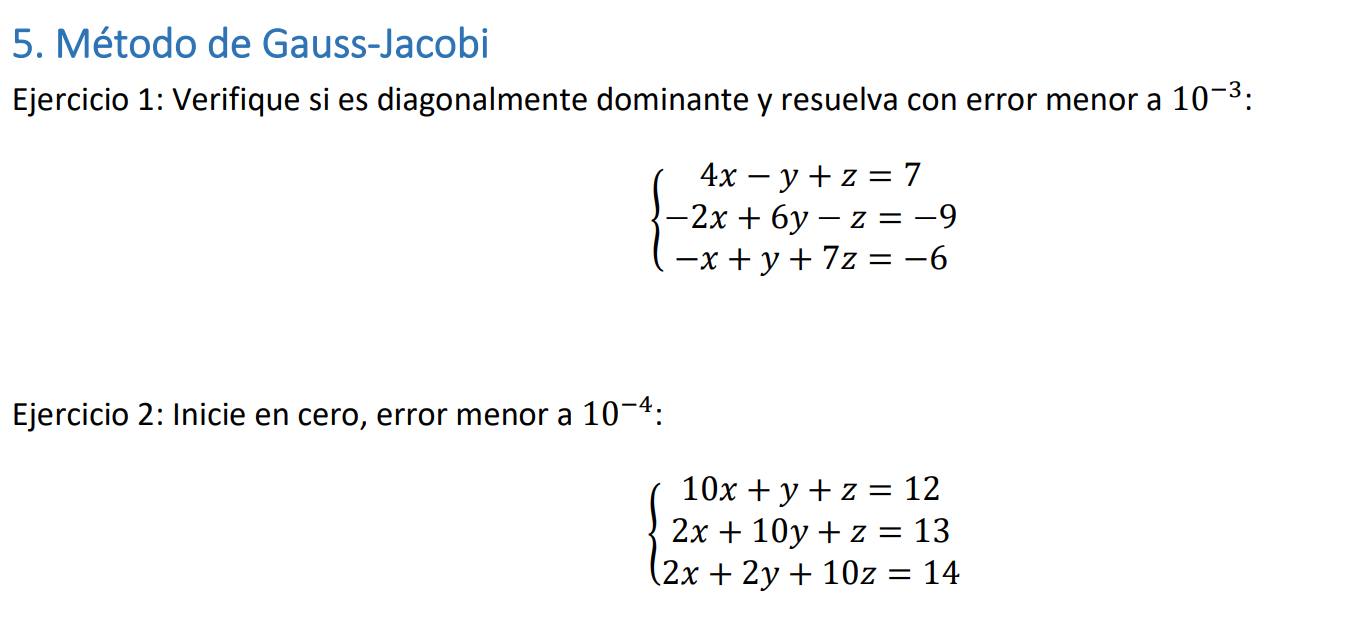
\includegraphics[width=1\textwidth]{./inFiles/Figures/Ej5.png}
\end{figure}

\textbf{a)}

$x = (7-z+y)/4$

$y = (-9+z+2x)/6$

$z = (-6+x-y)/7$

\begin{center}
\begin{tabular}{|c|c|c|}

\hline
x & y& z\\
\hline
0    & 0    & 0   \\
1.75   & -1.5    & -0.8571    \\
1.5893   & -1.0595    & -0.3929    \\
1.5759   & -1.0357    & -0.4787   \\
1.6108   & -1.0545    & -0.4791    \\
1.6062   & -1.0429    & -0.4764    \\
1.6083   & -1.0440    & -0.4787    \\
1.6087   & -1.0437    & -0.4782    \\
\hline
\end{tabular}
\end{center}

Calculamos max(1.6087   -1.0437    -0.4782)

Error Absoluto =$ \| 1.6083 - 1.6087\|$  = $4*10^{-4}$


\textbf{b)}

$x = (12-y-z)/10$

$y = (13-2x-z)/10$

$z = (14-2x-2y)/10$

\begin{center}
\begin{tabular}{|c|c|c|}

\hline
x & y& z\\
\hline
0    & 0    & 0   \\
1.2   & 1.3    & 1.4    \\
0.93   & 0.92    & 0.9    \\
1.018   & 1.024    & 1.03    \\
0.9946   & 0.9934    & 0.9904   \\
1.00162   & 1.00204    & 1.0024    \\
0.99956   & 0.99944   & 0.99927    \\
1.00013   & 1.0016    & 1.0002    \\
0.99996   & 0.99995    & 0.99994    \\
1.00001   & 1.00001    & 1.00002   \\
\hline
\end{tabular}
\end{center}

Calculamos max(1.00001  1.00001   1.00002 )

Error Absoluto =$ \| 1.00001 - 0.99996\|$  = $50*10^{-6}$

\begin{figure}[H]
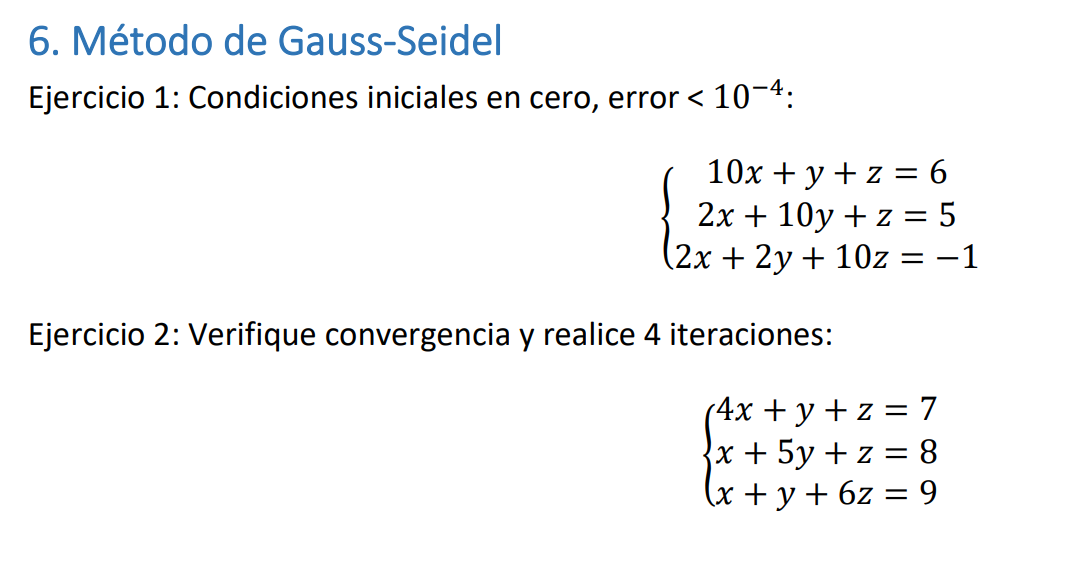
\includegraphics[width=1\textwidth]{./inFiles/Figures/Ej6.png}
\end{figure}

\textbf{a)}

$x = (6-y-z)/10$

$y = (5-2x-z)/10$

$z = (-1-2x-2y)/10$

\begin{center}
\begin{tabular}{|c|c|c|}

\hline
x & y& z\\
\hline
0    & 0    & 0   \\
0.6   & 0.38    & -0.296   \\
0.5916   & 0.41128    & -0.30058    \\
0.58893   & 0.41227    & -0.30024    \\
0.58880   & 0.41226    & -0.30021  \\
0.58880   & 0.41226     & -0.30021   \\

\hline
\end{tabular}
\end{center}

Calculamos max(0.58880  0.41226    -0.30021)

Error Absoluto =$ \| 0.58880 - 0.58880..\|$  = $5*10^{-6}$

\textbf{b)}

Si se puede porque es diagonal dominante

$x = (7-y-z)/4$

$y = (8-x-z)/5$

$z = (9-x-y)/6$

\begin{center}
\begin{tabular}{|c|c|c|}

\hline
x & y& z\\
\hline
0    & 0    & 0   \\
1.75  & 1.25    & 1   \\
1.1875   & 1.1625    & 1.1083    \\
1.1823   & 1.1418    & 1.1127    \\
1.1864   & 1.1402    & 1.1122  \\

\hline
\end{tabular}
\end{center}

Calculamos max(1.1864  1.1402   1.1122 )

Error Absoluto =$ \| 1.1864 - 1.1823\|$  = $4.1*10^{-3}$



\vspace{0.5cm}
\renewcommand{\refname}{\MakeUppercase{REFERENCIAS}}
\bibliographystyle{IEEEtran}
\bibliography{inFiles/References/references.bib}

\end{document}
